\documentclass[11pt]{article}
\usepackage[margin=1in]{geometry}
\usepackage{amsmath,amssymb}
\usepackage{tikz}
\usetikzlibrary{arrows.meta,positioning}
\usepackage{xcolor}
\pagestyle{empty}

\newcommand{\Wc}{\mathcal{W}}

\begin{document}
\begin{center}
{\Large NS Global Regularity — One-Page Roadmap}\\[4pt]
{\small A1–A6 = classical inputs; S1–S2 = novel statements proved in this manuscript}
\end{center}

\vspace{4mm}
\noindent\textbf{Statements (informal):}
\begin{itemize}
  \item A1 (\emph{Critical $\varepsilon$–regularity}). If $\displaystyle \Wc(x_0,t_0;r_0)\le \varepsilon_A$, then $\displaystyle \sup_{Q_{r_0/2}}|\omega|\lesssim r_0^{-2}\,\Wc^{2/3}$.
  \item A2 (\emph{Density–drop}). If $\Wc(0,0;1)\le \varepsilon_0+\eta$ ($\eta$ small) then $\Wc(0,0;\vartheta)\le \varepsilon_0+c\eta$.
  \item A3 (\emph{Carleson characterization of $BMO^{-1}$}). Heat–flow square function equivalence.
  \item A4 (\emph{Koch–Tataru small data}). $\|u_0\|_{BMO^{-1}}\le \varepsilon_{\mathrm{SD}}$ $\Rightarrow$ global mild solution, smooth for $t>0$.
  \item A5 (\emph{Backward/forward uniqueness}). Carleman backward uniqueness and forward energy uniqueness.
  \item A6 (\emph{Compactness/critical element}). Suitable solutions are compact locally in $L^3$; extract an ancient critical element; $\Wc$ semicontinuity.
  \item S1 (\emph{Slice bridge}). If $\sup_{(x,t),r}\Wc(x,t;r)\le \varepsilon$ on a unit window, then $\exists\,t_*:\ \|u(\cdot,t_*)\|_{BMO^{-1}}\lesssim \varepsilon^{2/3}$.
  \item S2 (\emph{Forward $\Wc$ gap}). If $\|u(\cdot,t_*)\|_{BMO^{-1}}\le \varepsilon$, then on $[t_*+c,\,t_*+1]$: $\sup_x\Wc(x,t;1)\lesssim \varepsilon^{3/2}$ (via local $BMO^{-1}\!\to L^3$ and $L^3\!\to L^{3/2}$ embeddings).
\end{itemize}

\vspace{2mm}
\begin{center}
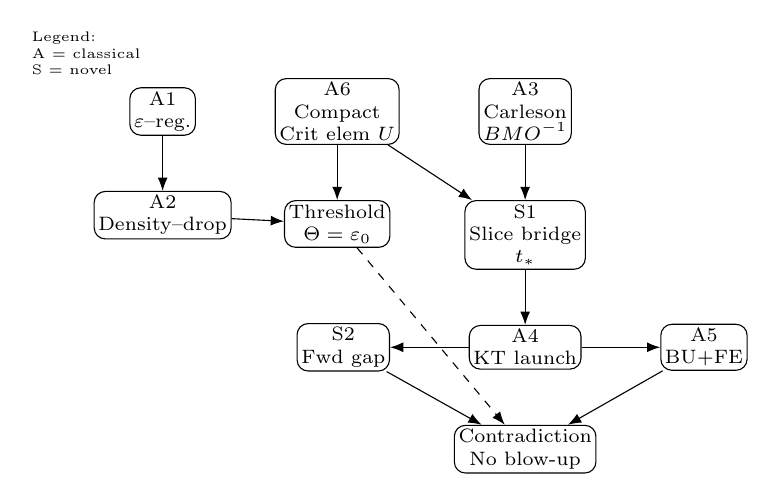
\begin{tikzpicture}[node distance=7mm and 10mm, every node/.style={draw, rounded corners, align=center, font=\scriptsize, inner sep=1.5pt}, >=Latex]
  % Top row
  \node (A1) {A1\\$\varepsilon$–reg.};
  \node (A6) [right=of A1] {A6\\Compact\\Crit elem $U$};
  \node (A3) [right=of A6] {A3\\Carleson\\$BMO^{-1}$};

  % Middle row
  \node (A2) [below=of A1] {A2\\Density–drop};
  \node (TC) [below=of A6] {Threshold\\$\Theta=\varepsilon_0$};
  \node (S1) [below=of A3] {S1\\Slice bridge\\$t_*$};

  % Bottom row
  \node (A4) [below=of S1] {A4\\KT launch};
  \node (S2) [left=of A4] {S2\\Fwd gap};
  \node (A5) [right=of A4] {A5\\BU+FE};
  \node (END) [below=of A4] {Contradiction\\No blow-up};

  % Edges
  \draw[->] (A1) -- (A2);
  \draw[->] (A6) -- (TC);
  \draw[->] (A2) -- (TC);
  \draw[->] (A6) -- (S1);
  \draw[->] (A3) -- (S1);
  \draw[->] (S1) -- (A4);
  \draw[->] (A4) -- (S2);
  \draw[->] (A4) -- (A5);
  \draw[->] (S2) -- (END);
  \draw[->] (A5) -- (END);
  \draw[->, dashed] (TC) -- (END);

  % Legend
  \node[draw=none, align=left, font=\tiny] (LEG) [above left=1mm and -2mm of A1] {Legend:\\A = classical\\S = novel};
\end{tikzpicture}
\end{center}

\vspace{2mm}
\noindent\textbf{Flow of the proof (one line).}\quad Assume first blow-up $\Rightarrow$ extract ancient critical element $U$ (A6); density–drop pins $\mathcal M_c=\varepsilon_0$ (A1,A2); slice bridge gives small $BMO^{-1}$ at some $t_*$ (S1,A3); launch KT flow (A4) and obtain a forward $\Wc$ gap (S2); backward/forward uniqueness identifies $U$ with the smooth flow on $[t_*,0]$ and contradicts saturation at $(0,0;1)$ (A5).

\end{document}


